The Xedef Courier Company provides air package delivery among several cities. Some of these cities are Xedef hubs where special processing facilities are established. Each of Xedef's aircraft shuttles back and forth between one pair of cities, carrying packages in either direction as required.  

To be shipped from one city to another, a package must be transported by a sequence of hops, where each hop carries the package between a pair of cities served by one of the
aircraft. Furthermore, the sequence must include at least one of Xedef's hubs.

To facilitate routing, Xedef wishes to encode the length of the shortest sequence of
hops from every city to every hub on the shipping label of every package. (The length
of the shortest sequence leading from a hub to itself is zero.) Obviously, a compact
representation of this information is required. 

You are to implement two procedures, \t{encode(N,H,P,A,B)} and \t{decode(N,H)}. $N$ is the number of cities and $H$ is the number of hubs. Assume that the cities are numbered
from $0$ to $N-1$, and that the hubs are the cities with numbers between $0$ and $H-1$.
Further assume that $N \le 1000$ and $H \le 36$. $P$ is the number of pairs of cities connected by aircraft. All (unordered) pairs of cities will be distinct. $A$ and $B$ are arrays of size $P$, such that the first pair of connected cities is $(A[0], B[0])$, the second pair is $(A[1], B[1])$, and so on.

\t{encode} must compute a sequence of bits from which decode can determine the
number of hops from every city to every hub. \t{encode} will transmit the sequence of
bits to the grading server by a sequence of calls to \t{encode\_bit(b)} where \t{b} is either $0$ or $1$. 

\t{decode} will receive the sequence of bits from the grading server by making calls
to \t{decode\_bit}. The $i$-th call to \t{decode\_bit} will return the value of $b$ from the $i$-th call to \t{encode\_bit(b)}. Note that you must ensure that the number of
times \t{decode} calls \t{decode\_bit} will always be at most equal to the number of
times \t{encode} previously called \t{encode\_bit(b)}.

After decoding the numbers of hops, decode must call \t{hops(h,c,d)} for every
hub $h$ and every city $c$ (including every hub, that is, also for $c=h$), giving the
minimum number $d$ of hops necessary to ship a package between $h$ and $c$. That is,
there must be $N*H$ calls to \t{hops(h,c,d)}. The order does not matter. You are 
guaranteed that it is always possible to ship a package between every hub and every
city.

On original IOI you need to submit 2 separate files with \t{encode} and \t{decode} function, but here they must be implemented in one file. Anyway, between calling \t{encode} and \t{decode} your solution would be restarted, so no data could be saved. They must communicate only using \t{encode\_bit}/\t{decode\_bit} functions. But for simplicity of testing, provided version of grader would call both functions in the same run. 


As an example, consider the following diagram:

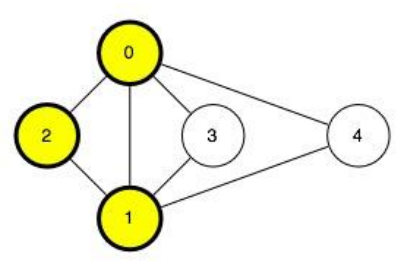
\includegraphics{SaveitSample.png}

It shows five cities $N=5$ connected by seven aircraft $P=7$. Cities $0$, $1$ and $2$ are hubs $H=3$. One hop is needed to ship a package between hub $0$ and city $3$, whereas two hops are needed to ship a package between hub $2$ and city $3$. The entries in the following table are all $d$-values that decode must deliver by calling \t{hops(h,c,d)}:

\begin{tabular}{|l|l|l|l|l|l|}
\hline
  & 0 & 1 & 2 & 3 & 4 \\ \hline
0 & 0 & 1 & 1 & 1 & 1 \\ \hline
1 & 1 & 0 & 1 & 1 & 1 \\ \hline
2 & 1 & 1 & 0 & 2 & 2 \\ \hline
\end{tabular}

